\section{质因数分解}

\subsection{题目要求}

由用户输入一个十进制正整数 $N(2 \le N \le 4294967295)$,程序需要能够将该数字分解质因数之后输出他的各个因子。

\begin{itemize}
  \item 例1:输入 \verb|11|,输出 \verb|11 = 11|;
  \item 例2:输入 \verb|120|,输出 \verb|120 = 2 x 2 x 2 x 3 x 5|。
\end{itemize}

首先我们可以看出,用户输入的正整数 $N$ 很明显超出了 16 位数字的范围,因此我们有必要将运算的所有过程都扩展成 32 位无符号数的操作。

简单分析之后可以知道,对于这个问题我们需要实现以下若干模块:

\begin{enumerate}
  \item 将字符串解析为 32 位无符号数;
  \item 实现 32 位无符号数与 16 位无符号数的加法运算;
  \item 实现 32 位无符号数与 16 位无符号数的乘法运算;
  \item 实现 32 位无符号数与 16 位无符号数的除法运算;
  \item 将 32 位无符号数以十进制形式输出到控制台;
  \item 实现 32 位无符号数分解质因数。
\end{enumerate}

以下将会详细解释各个模块的设计过程以及参考代码。

\subsection{关键部分程序流程图}

\subsubsection{将字符串解析为 32 位无符号数}

\begin{figure}
  \centering
  \begin{tikzpicture}[node distance=2cm]
    \node (start) [startstop] {开始};
    \node (proc1) [process, below of=start] {$x \leftarrow 0$};
    \node (dec1)  [decision, below of=proc1, yshift=-1.5cm] {字符串是否读完};
    \node (proc2) [process, below of=dec1, yshift=-1.5cm] {令 $c$ 为当前字符};
    \node (dec2)  [decision, below of=proc2, yshift=-1cm] {$c$ 是否合法};
    \node (proc3) [process, below of=dec2, yshift=-1cm] {$x \leftarrow x \times 10$ \\ $x \leftarrow x + c - 48$};
    \node (proc4) [process, below of=proc3] {移动到字符串下一个字符};
    \node (echar) [io, right of=dec2, xshift=2.5cm] {输出错误:输入字符不合法};
    \node (stop)  [startstop, right of=proc3, xshift=2.5cm] {结束程序};
    \node (retn)  [startstop, right of=dec1, xshift=2.5cm] {返回结果 $x$};

    \draw [arrow] (start) -- (proc1);
    \draw [arrow] (proc1) -- (dec1);
    \draw [arrow] (dec1)  -- node[anchor=east] {No} (proc2);
    \draw [arrow] (dec1)  -- node[anchor=south] {Yes} (retn);
    \draw [arrow] (proc2) -- (dec2);
    \draw [arrow] (dec2)  -- node[anchor=east] {Yes} (proc3);
    \draw [arrow] (dec2)  -- node[anchor=south] {No} (echar);
    \draw [arrow] (proc3) -- (proc4);
    \node (p1) [shape=coordinate, left of=proc4, xshift=-1.5cm] {};
    \draw (proc4) -- (p1);
    \draw [arrow] (p1) |- (dec1);
    \draw [arrow] (echar) -- (stop);
  \end{tikzpicture}
  \caption{将字符串转化为无符号整数的流程图}
  \label{fig:atoi}
\end{figure}

将字符串转化为无符号整数的过程是一个非常经典的问题。
我们可以预先初始化一个变量 $x$,令其初值为 $0$。
之后每次读入一个字符 $c$,然后将该字符从 ASCII 码转换为对应的数字 $c'$,接着令 $x \leftarrow x \times 10 + c'$ 即可。
当读完了字符串之后 $x$ 便是我们想要的结果。
具体过程可以参考图 \ref{fig:atoi}。

值得注意的是如果运算过程中出现加法溢出,则表明用户输入的数字过大,这个时候可以检测出错误并且安全退出程序。

\subsubsection{32 位无符号数与 16 位无符号数的加法}

要计算 32 位无符号数与 16 位无符号数的加法则特别简单,只需要先将 32 位无符号数的低 16 位与另外一个数字相加,如果发现有溢出则将 32 位无符号数的高 16 位加一即可。
在汇编之中,我们可以简单地利用 \verb|add| 和 \verb|adc| 指令就可以实现我们需要的功能。

\subsubsection{32 位无符号数与 16 位无符号数的乘法}

\begin{figure}
  \centering
  \begin{tikzpicture}[node distance=2cm]
    \node (start) [startstop] {开始};
    \node (proc1) [process, large, below of=start] {$(H, L) \leftarrow A$};
    \node (proc2) [process, large, below of=proc1] {$(H_A, H_B) \leftarrow H \times B$ \\ $(L_A, L_B) \leftarrow L \times B$};
    \node (proc3) [process, large, below of=proc2] {$Ans \leftarrow (H_B + L_A, L_B)$};
    \node (stop) [startstop, below of=proc3] {返回乘法的结果 $Ans$};

    \draw [arrow] (start) -- (proc1);
    \draw [arrow] (proc1) -- (proc2);
    \draw [arrow] (proc2) -- (proc3);
    \draw [arrow] (proc3) -- (stop);
  \end{tikzpicture}
  \caption{32 位无符号数与 16 位无符号数的乘法流程图}
  \label{fig:dword_mul_word}
\end{figure}

将 32 位无符号数与 16 位无符号数的乘法则需要分为两步。
首先我们在汇编之中有一个指令 \verb|mul|,可以用于实现两个 16 位无符号数的乘法,结果可以得到一个 32 位的整数。
利用这个指令,我们可以先将 32 位无符号数拆分成高 16 位和低 16 位,然后分别与另一个数字相乘,最后将结果用加法加起来即可。
具体的计算过程可以参考图 \ref{fig:dword_mul_word}。

\subsubsection{32 位无符号数与 16 位无符号数的除法}

\begin{figure}
  \centering
  \begin{tikzpicture}[node distance=2cm]
    \node (start) [startstop] {开始};
    \node (proc1) [process, large, below of=start] {$(H, L) \leftarrow A$};
    \node (proc2) [process, large, below of=proc1] {$(S_H, R_H) \leftarrow (0, H) / B$ \\ $(S_L, R_L) \leftarrow (R_H, L) / B$};
    \node (proc3) [process, large, below of=proc2] {$S \leftarrow (S_H, S_L)$ \\ $R \leftarrow R_L$};
    \node (stop) [startstop, below of=proc3] {返回商 $S$ 和余数 $R$};

    \draw [arrow] (start) -- (proc1);
    \draw [arrow] (proc1) -- (proc2);
    \draw [arrow] (proc2) -- (proc3);
    \draw [arrow] (proc3) -- (stop);
  \end{tikzpicture}
  \caption{32 位无符号数与 16 位无符号数的除法流程图}
  \label{fig:dword_div_word}
\end{figure}

计算 32 位无符号数与 16 位无符号数的除法操作的基本思想也与乘法类似。
汇编中提供了 \verb|div| 指令可以用来计算 32 位无符号数除以 16 位无符号数的结果,但是除法的商只能计算 16 位。
因此我们依旧只能将 32 位无符号数拆分成两个 16 位的无符号数字,之后依次进行除法运算。
具体的计算过程可以参考图 \ref{fig:dword_div_word}。

\subsubsection{输出 32 位无符号数}

输出 32 位无符号数大致需要两个步骤,第一步是将整数划分成十进制下的各个数位,第二步则是将其打印到控制台输出。

\begin{figure}
  \centering
  \begin{tikzpicture}[node distance=2cm]
    \node (start) [startstop] {开始};
    \node (prepare) [process, below of=start] {$a \leftarrow \varnothing $};
    \node (dec1) [decision, below of=prepare] {$x > 0$};
    \node (proc1) [process, below of=dec1] {$S, R \leftarrow x / 10$};
    \node (proc2) [process, below of=proc1] {$x \leftarrow S$ \\ $a \leftarrow a \cap \{R\}$};
    \node (proc3) [process, right of=dec1, xshift=3cm] {翻转 $a$};
    \node (output) [io, text width=2.5cm, below of=proc3] {输出字符串 $a$};
    \node (stop) [startstop, below of=output] {结束};

    \draw [arrow] (start) -- (prepare);
    \draw [arrow] (prepare) -- (dec1);
    \draw [arrow] (dec1) -- node[anchor=east] {Yes} (proc1);
    \draw [arrow] (dec1) -- node[anchor=south] {No} (proc3);
    \draw [arrow] (proc1) -- (proc2);
    \node (p1) [shape=coordinate, left of=proc2, xshift=-1.5cm] {};
    \draw (proc2) -- (p1);
    \draw [arrow] (p1) |- (dec1);
    \draw [arrow] (proc3) -- (output);
    \draw [arrow] (output) -- (stop);
  \end{tikzpicture}
  \caption{32 位无符号数以十进制输出的流程图}
  \label{fig:print_dword_dec}
\end{figure}

对于第一步来说,我们只需要每次将数字 $x$ 整除 $10$ 并取余数,那么我们就可以得到数字 $x$ 在十进制下各个数位的值。
但是值得注意的是我们需要输出的顺序和每次整除取余的顺序是相反的,因此我们有必要预先将每个数字都求出来,并在最后将整个字符串翻转一下再输出。
具体的计算过程可以参考图 \ref{fig:print_dword_dec}

\subsubsection{分解质因数}

\begin{figure}
  \centering
  \begin{tikzpicture}[node distance=2cm]
    \node (start) [startstop] {开始};
    \node (prepare) [process, below of=start] {$p \leftarrow 2$};
    \node (dec1) [decision, below of=prepare] {$n > 1$};
    \node (dec2) [decision, below of=dec1, yshift=-1cm] {$n \bmod p = 0$};
    \node (op) [io, text width=2.5cm, below of=dec2, yshift=-1cm] {输出素因子 $p$};
    \node (proc1) [process, below of=op] {$n \leftarrow n / p$};
    \node (proc2) [process, below of=proc1] {$p \leftarrow p + 1$};
    \node (dec3) [decision, below of=proc2, yshift=-0.5cm] {$p \ge 2^{16}$};
    \node (dec4) [decision, below of=dec3, yshift=-0.5cm] {$n > 1$};
    \node (on) [io, text width=2.5cm, below of=dec4] {输出素因子 $n$};
    \node (stop) [startstop, below of=on] {结束};

    \node (p1) [shape=coordinate, left of=proc1, xshift=-1.5cm] {};
    \node (p2) [shape=coordinate, right of=dec2, xshift=1.5cm] {};
    \node (p3) [shape=coordinate, left of=dec3, xshift=-2.5cm] {};
    \node (p4) [shape=coordinate, right of=dec1, xshift=2.5cm] {};
    \node (p5) [shape=coordinate, left of=dec4, xshift=-2.5cm] {};

    \draw [arrow] (start) -- (prepare);
    \draw [arrow] (prepare) -- (dec1);
    \draw (proc1) -- (p1);
    \draw [arrow] (p1) |- (dec2);
    \draw [arrow] (op) -- (proc1);
    \draw [arrow] (proc2) -- (dec3);
    \draw [arrow] (dec2) -- node[anchor=east] {Yes} (op);
    \draw (dec2) -- node[anchor=south] {No} (p2);
    \draw [arrow] (p2) |- (proc2);
    \draw (dec3) -- node[anchor=south] {No} (p3);
    \draw [arrow] (p3) |- (dec1);
    \draw (dec1) -- node[anchor=south] {No} (p4);
    \draw [arrow] (p4) |- (stop);
    \draw [arrow] (dec1) -- node[anchor=east] {Yes} (dec2);
    \draw [arrow] (dec3) -- node[anchor=east] {Yes} (dec4);
    \draw [arrow] (dec4) -- node[anchor=east] {Yes} (on);
    \draw [arrow] (on) -- (stop);
    \draw (dec4) -- node[anchor=south] {No} (p5);
    \draw [arrow] (p5) |- (stop);
  \end{tikzpicture}
  \caption{分解质因数的算法}
  \label{fig:factor}
\end{figure}

我们采用经典的 $O(\sqrt{n})$ 的算法来分解质因数。考虑经典的枚举素因子来分解 $n$ 的算法,显然当我们将素因子枚举到 $\sqrt{n}$ 的时候便可以停止继续枚举,因为 $n$ 必不可能同时含有两个大于 $\sqrt{n}$ 的素因子存在。因此此时如果 $n$ 仍然没有被除尽,则可以直接判定剩下的结果必然为最大的一个素因子。整个分解的过程可以参考图 \ref{fig:factor}。

\subsection{关键部分的源代码}

\subsubsection{若干宏定义}

首先我们有若干个宏定义来简化我们的代码。

\begin{lstlisting}[language={[x86masm]Assembler},morekeywords={}]
.data
crlf    db      0dh, 0ah, "$"  ; 回车换行
.code
; print 宏,用于输出 msg 到控制台
print   macro   msg
        mov     ah, 09h         ; AH=09h 为执行打印字符串的功能
        mov     dx, offset msg  ; 传入字符串起始地址
        int     21h             ; 调用 21h 中断执行操作
        endm

; println 宏,用于输出 msg 到控制台并换行
println   macro   msg
          print   msg
          print   crlf
          endm

; exit 宏,用于结束整个程序
exit    macro   code
        mov     ah, 4ch         ; AH=4ch 为执行推出程序的操作
        mov     al, code        ; 传入程序的退出状态码
        int     21h             ; 调用 21h 中断执行操作
        endm

; panic 宏,用于输出错误信息到控制台并退出程序
panic   macro   errmsg, code
        println errmsg
        exit    code
        endm
\end{lstlisting}

另外,我们有 \verb|gets| 子程序用来从控制台读入一行字符串,有点类似 C 语言中的 \verb|gets| 函数,故取名之。\verb|gets| 子程序的结果会直接写入到 \verb|data| 段的 \verb|rdsz|、\verb|strlen| 和 \verb|rdstr| 中。

\begin{lstlisting}[language={[x86masm]Assembler},morekeywords={}]
.data
rdsz    db      255            ; 读入缓冲区大小
strlen  db      ?              ; 读入字符串长度
rdstr   db      255 dup(0)     ; 读入缓冲区
.code
gets    proc
        mov     ah, 0ah         ; AH=0ah 表示从控制台中读取一行字符串
        mov     dx, offset rdsz ; 传入参数地址
        int     21h             ; 调用中断执行操作
        print   crlf            ; 打印换行
        ret                     ; 返回到原程序
gets    endp
\end{lstlisting}

\subsubsection{32 位无符号数与 16 位无符号数的乘法 u32mul}

\verb|u32mul| 子程序用于计算 32 位无符号数与 16 位无符号数的乘法运算。其中 32 位无符号数从 \verb|BX| 寄存器传入地址,16 位无符号数从 \verb|AX| 寄存器传入。结果将直接写回到 \verb|BX| 寄存器的地址中。

\begin{lstlisting}[language={[x86masm]Assembler},morekeywords={}]
.data
enumlg  db      "error: number is too large", "$"
.code
; 计算 dword ptr [bx] *= ax
u32mul  proc
        push    bp
        mov     bp, sp            ; 保存环境
        sub     sp, 10            ; 保留 10 字节
        mov     [bp-2], ax        ; 保存乘数 AX 的值
        mov     ax, ss:[bx]       ; 将低 16 位放入 AX
        mul     word ptr [bp-2]   ; 计算低 16 位与乘数相乘的结果
        mov     [bp-4], dx        ; 将结果的高 16 位存入栈中
        mov     [bp-6], ax        ; 将结果的低 16 位存入栈中
        mov     ax, ss:[bx+2]     ; 将高 16 位放入 AX
        mul     word ptr [bp-2]   ; 计算高 16 位与乘数相乘的结果
        jc      u32muloverflow    ; 如果 CF = 1,则说明结果溢出
        mov     [bp-8], dx        ; 将结果的高 16 位存入栈中
        mov     [bp-10], ax       ; 将结果的低 16 位存入栈中
        mov     ax, [bp-4]        ; 结果的高 16 位为 [bp-4] + [bp-10]
        add     ax, [bp-10]       ; 直接在 AX 中计算加法
        jc      u32muloverflow    ; 如果加法出现溢出,说明结果溢出
        mov     ss:[bx+2], ax     ; 将加法结果存回 [BX]
        mov     ax, [bp-6]        ; 结果的低 16 位即为 [bp-6]
        mov     ss:[bx], ax
        mov     sp, bp            ; 恢复环境
        pop     bp
        ret                       ; 返回到原程序
u32muloverflow:
        panic   enumlg, 1         ; 乘法出现溢出,结束程序
u32mul  endp
\end{lstlisting}

\subsubsection{32 位无符号数与 16 位无符号数的除法 u32div}

\verb|u32div| 子程序用于计算 32 位无符号数与 16 位无符号数的除法结果。与 \verb|u32mul| 子程序类似,32 位无符号数通过 \verb|BX| 寄存器传入地址,除数则通过 \verb|AX| 寄存器传入。结果会直接写回到 \verb|BX| 寄存器指向的地址中,另外余数将会保留到 \verb|DX| 寄存器中。

\begin{lstlisting}[language={[x86masm]Assembler},morekeywords={}]
; 计算 dword ptr [bx] /= ax,余数保存在 DX
u32div  proc
        push    bp
        mov     bp, sp          ; 保存环境
        sub     sp, 2           ; 保留 2 个字节用于存放数据
        mov     [bp-2], ax      ; 保存除数到栈空间中
        mov     dx, 0
        mov     ax, ss:[bx+2]
        div     word ptr [bp-2] ; 计算 (0, [BX+2]) 做除法的结果
        mov     ss:[bx+2], ax   ; 将结果的商写回到 [BX+2] 中
        mov     ax, ss:[bx]     ; 此时余数保留在 DX 中
        div     word ptr [bp-2] ; 计算 (DX, [BX]) 做除法的结果
        mov     ss:[bx], ax     ; 将结果的商写回到 [BX] 中
                                ; 整个结果的余数保存在 DX 中
        mov     sp, bp          ; 恢复环境
        pop     bp
        ret                     ; 返回到原程序
u32div  endp
\end{lstlisting}

\subsubsection{以十进制读入 32 位无符号数 r32dec}

\begin{lstlisting}[language={[x86masm]Assembler},morekeywords={}]
.data
einvch  db      "error: invalid charactor", "$"
.code
; 从 rdstr 中以十进制解析字符串
; 结果将会放在 dword ptr [bx] 中 
r32dec  proc
        push    si
        push    cx
        push    bp
        mov     bp, sp          ; 保护环境
        mov     word ptr ss:[bx+2], 0   ; 初始化 dword ptr [bx] 为 0
        mov     word ptr ss:[bx], 0
        mov     si, 0           ; si = 当前字符串中读入的下标
        mov     cx, 0           ; cx = 循环次数(字符串长度)
        mov     cl, strlen
        jcxz    rdscanend       ; 如果 cx = 0 则直接跳转到循环结束
rdscan:
        mov     ax, 0ah         ; 传入乘数 10
        call    u32mul          ; 计算 dword ptr [bx] *= 10
        mov     ax, 0           ; AX 置零
        mov     al, rdstr[si]   ; 读入当前字符到 AL 中
        cmp     al, 30h
        jb      rdeinvch        ; 如果 AL < '0' 则为非法字符
        cmp     al, 39h
        ja      rdeinvch        ; 如果 AL > '9' 则为非法字符
        xor     al, 30h         ; 将 AL 从 ASCII 码转化为数字
        add     word ptr ss:[bx],     ax   ; 计算 dword ptr [bx] += ax
        adc     word ptr ss:[bx+2],   0    ; 处理进位
        jc      rdeovfl         ; 如果计算结果溢出则表述读入的数字超出了范围
        inc     si              ; 移动到下一个字符
        loop    rdscan          ; 循环读入字符
rdscanend:
        mov     sp, bp          ; 恢复环境
        pop     bp
        pop     cx
        pop     si
        ret                     ; 返回到原程序
rdeinvch:
        panic   einvch, 1       ; 输出非法字符并退出
rdeovfl:
        panic   enumlg, 1       ; 输出输入数字溢出并退出
r32dec  endp
\end{lstlisting}

\subsubsection{十进制输出 32 位无符号数 w32dec}

\verb|w32dec| 用于将一个 32 位无符号数以十进制输出到控制台中。32 位无符号数的地址通过 \verb|BX| 寄存器传入,不会修改原来值。

\begin{lstlisting}[language={[x86masm]Assembler},morekeywords={}]
.data
wrtbuf  db      100 dup(0)      ; 输出缓冲区
.code
; 将 dword ptr [bx] 以十进制格式输出
w32dec  proc
        push    ax
        push    cx
        push    dx
        push    si
        push    di
        push    bp
        mov     bp, sp          ; 保存环境
        sub     sp, 4           ; 保留 4 字节保存变量
        mov     ax, ss:[bx+2]   ; 复制 dword ptr [bx] 到 dword ptr [bp-4]
        mov     [bp-2], ax      ; 以下不妨令 dword ptr [bp-4] 为 x
        mov     ax, ss:[bx]
        mov     [bp-4], ax
        mov     di, 0           ; 初始化字符串的长度为 0
w32decdivwhile:
        cmp     word ptr [bp-2], 0
        jne     w32decdivbody   ; 如果 x != 0 则继续进行除法
        cmp     word ptr [bp-4], 0
        jne     w32decdivbody   ; 如果 x != 0 则继续进行除法
        jmp     w32decdivend    ; 如果 x = 0 则跳出循环
w32decdivbody:
        lea     bx, [bp-4]      ; 传入 BX 参数
        mov     ax, 0ah         ; 传入除数 10
        call    u32div          ; 调用除法子程序
        mov     ax, dx          ; 将余数保存到 AX 中
        xor     al, 30h         ; 将 AL 从数字转换成 ASCII 码
        mov     wrtbuf[di], al  ; 将字符添加到字符串的最后
        inc     di              ; 字符串长度 ++
        jmp     w32decdivwhile  ; 返回循环
w32decdivend:
        test    di, di          ; 如果 di = 0 则需要额外添加一个 0 字符
        jnz     w32decadddollar ; 如果 di != 0 则不需要
        mov     wrtbuf[di], 30h ; 在字符串结尾添加一个 '0' 字符
        inc     di              ; 字符串长度 ++
w32decadddollar:
        mov     wrtbuf[di], 24h ; 在字符串最后添加 '$' 符号
        mov     si, 0           ; 令 si 为 0
        dec     di              ; 另 di 为字符串数字部分的最大下标
        jz      w32decrevend    ; 如果 si = di = 0 则不需要翻转
w32decrevloop:
        mov     al, wrtbuf[di]  ; 交换 wrtbuf[si] 和 wrtbuf[di]
        xchg    al, wrtbuf[si]
        mov     wrtbuf[di], al
        inc     si              ; si ++
        dec     di              ; di --
        cmp     si, di
        jb      w32decrevloop   ; 如果 si < di 则要继续交换
w32decrevend:
        print   wrtbuf          ; 输出字符串到控制台
        mov     sp, bp          ; 恢复环境
        pop     bp
        pop     di
        pop     si
        pop     dx
        pop     cx
        pop     ax
        ret                     ; 返回到原程序
w32dec  endp
\end{lstlisting}

\subsubsection{分解质因数 factor}

\verb|factor| 子程序用于将给定的 32 位无符号数分解质因数并且打印到控制台中。其中 32 位无符号数的地址使用 \verb|BX| 寄存器给出。

\begin{lstlisting}[language={[x86masm]Assembler},morekeywords={}]
.data
equal   db      " = ", "$"
times   db      " x ", "$"
.code
factor  proc
        push    bp
        mov     bp, sp                ; 保存环境
        sub     sp, 10                ; 保留 10 个字节的空间
        ; 栈上的 10 个字节空间分配如下
        ; n     dword   [bp-4]
        ; p     word    [bp-6]
        ; m     dword   [bp-10]
        mov     ax, ss:[bx+2]         ; 将 [BX] 中的数字复制到 n 中
        mov     [bp-2], ax
        mov     ax, ss:[bx]
        mov     [bp-4], ax
        mov     word ptr [bp-6], 2    ; 初始化 p = 2
        lea     bx, [bp-4]            ; 给出 n 的地址
        call    w32dec                ; 将 n 打印到控制台
        mov     cx, 0                 ; cx = 0 表示当前为第一个素因子
factorloop:
        cmp     word ptr [bp-2], 0
        ja      factorloopbody        ; 如果 n > 1 则继续分解因子
        cmp     word ptr [bp-4], 1
        ja      factorloopbody        ; 如果 n > 1 则继续分解因子
        jmp     factorloopbreak       ; 否则分解质数完成
factorloopbody:
        mov     ax, [bp-2]            ; 复制 n 到 m 中
        mov     [bp-8], ax
        mov     ax, [bp-4]
        mov     [bp-10], ax
        lea     bx, [bp-10]           ; 给出被除数 m 的地址
        mov     ax, [bp-6]            ; 给出除数 p
        call    u32div                ; 计算除法
        test    dx, dx                ; DX 保存除法的余数
        jnz     factorloopcontinue    ; 如果余数不为 0 则跳出循环
        mov     ax, [bp-8]            ; 将除法的商从 m 复制回 n 中
        mov     [bp-2], ax
        mov     ax, [bp-10]
        mov     [bp-4], ax
        jcxz    factorloopcxzthen     ; 如果当前是否是第一个素因子
        print   times                 ; 如果不是则打印 " x "
        jmp     factorloopcxzend
factorloopcxzthen:
        print   equal                 ; 如果是则打印 " = "
        inc     cx                    ; 取消第一个素因子的标记
factorloopcxzend:
        lea     bx, [bp-6]            ; 给出素因子 p 的地址
        call    w16dec                ; 打印 16 位无符号数到控制台
        jmp     factorloopbody        ; 继续尝试能否整除
factorloopcontinue:
        inc     word ptr [bp-6]       ; p ++
        jnz     factorloop            ; 如果 p 没有越界,则继续尝试除法
factorloopbreak:
        cmp     word ptr [bp-2], 0    ; 如果 p 越界,则判断是否 n > 1
        ja      factorendprime        ; 如果 n > 1 跳转输出
        cmp     word ptr [bp-4], 1
        ja      factorendprime        ; 如果 n > 1 跳转输出
        jmp     factorend             ; 否则可以结束子程序
factorendprime:
        jcxz    factorcxzthen         ; 判断是否为第一个素因子
        print   times                 ; 如果不是则打印 " x "
        jmp     factorcxzend
factorcxzthen:
        print   equal                 ; 如果是则打印 " = "
        inc     cx                    ; 并且取消第一个素因子的标记
factorcxzend:
        lea     bx, [bp-4]            ; 给出 n 的地址
        call    w32dec                ; 打印 n 到控制台
factorend:
        print   crlf                  ; 换行
        mov     sp, bp                ; 恢复环境
        pop     bp
        ret                           ; 返回到原程序
factor  endp
\end{lstlisting}

其中代码中有出现 \verb|w16dec| 子程序,该子程序仅用于在栈空间中多申请一个字节并且调用 \verb|w32dec| 来显示原本为 16 位的无符号数。

\begin{lstlisting}[language={[x86masm]Assembler},morekeywords={}]
w16dec  proc
        push    bp
        mov     bp, sp        ; 保护环境
        sub     sp, 4         ; 保留 4 字节的空间
        mov     ax, 0         ; 将高字节置零
        mov     [bp-2], ax
        mov     ax, ss:[bx]   ; 将低字节复制 [BX] 的值
        mov     [bp-4], ax
        lea     bx, [bp-4]    ; 给出栈中的地址
        call    w32dec        ; 调用 32 位无符号数的十进制输出子程序
        mov     sp, bp        ; 恢复环境
        pop     bp
        ret                   ; 返回到原程序
w16dec  endp
\end{lstlisting}

\subsubsection{主程序 \_start}

整个程序从 \verb|_start| 开始运行。整个程序的过程大体分为三步:读入、解析、分解质因数并输出。

\begin{lstlisting}[language={[x86masm]Assembler},morekeywords={}]
.data
enumsm  db      "error: number is too small", "$"
.code
_start  proc
        mov     ax, @data
        mov     ds, ax          ; 初始化 DS 为数据段
        mov     es, ax          ; 初始化 ES 为数据段
        mov     bp, sp          ; 初始化 bp 为栈顶地址
        sub     sp, 4           ; 保留 4 个字节用于存放操作数
        call    gets            ; 调用 gets 子程序读入一行字符串
        lea     bx, [bp-4]      ; 给出希望存放解析结果的地址
        call    r32dec          ; 调用十进制解析子程序
        cmp     word ptr [bp-2], 0
        ja      continue        ; 如果 x > 1 则继续
        cmp     word ptr [bp-4], 1
        ja      continue        ; 如果 x > 1 则继续
        panic   enumsm, 1       ; 否则输出错误信息并退出
continue:
        lea     bx, [bp-4]      ; 给出希望分解质因数的数据地址
        call    factor          ; 调用分解质因数子程序
        exit    0               ; 结束程序
_start  endp

end     _start
\end{lstlisting}

\subsection{运行结果及分析}

\begin{figure}[h]
  \centering
  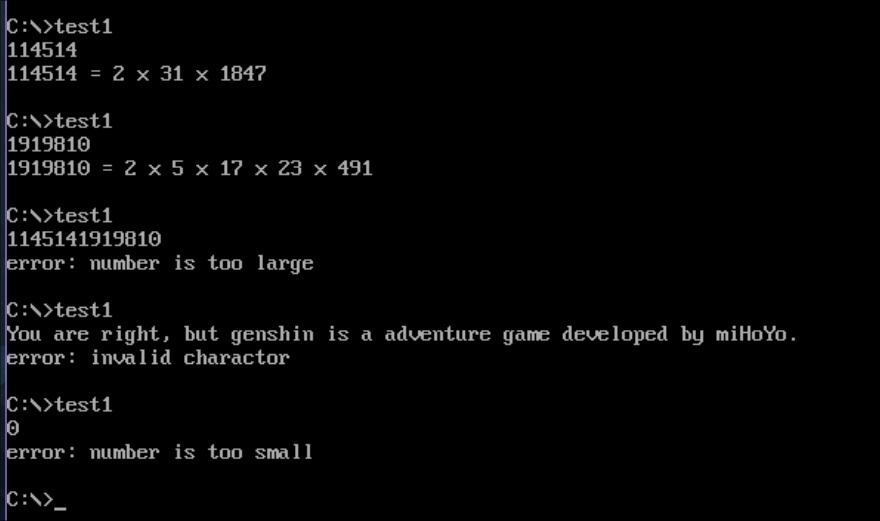
\includegraphics[width=300pt]{figure/test1res.png}
  \caption{运行结果}
  \label{fig:result1}
\end{figure}

从图 \ref{fig:result1} 中可以看到对于程序的五次运行测试。其中前两次测试都输入了正确的数字,并且可以看到程序可以正确地处理所有步骤并且输出了正确的结果。第三次测试中我们输入了一个超出数据范围的数字,程序会提示数据超出范围,并且及时停止了程序的运行。第四次测试中我们输入了非法的内容,程序会提示解析到非法字符,并且终止了程序的运行。第五次我们输入了一个比数据范围还要小的数字,程序会提示数据过小,并且直接退出。

\subsection{遇到的问题及解决办法}

在实现代码的过程中也遇到了很多的问题,不过大部分都可以通过参阅 8086 CPU 的指令集文档解决。

其中值得一提的是使用 \verb|[BX]| 来获取数据的时候默认使用的是 \verb|DS| 数据段寄存器来定位,然而我们在编写代码的过程中传递操作数的时候基本都是直接在栈中开辟内存空间来存放数据的。因此我们在每个使用 \verb|BX| 来间接寻址的地方都要在前面加上 \verb|SS:| 来强制使用 \verb|SS| 寄存器作为我们的段基地址。

另外,对于一些操作数分别为内存地址和立即数的指令,编译器可能无法有效推断出操作数的类型。这时候我们也需要手动使用 \verb|word ptr| 或者 \verb|dword ptr| 来显示声明操作数的类型。
